% Copyright (c)  2019  FSC.
% Permission is granted to copy, distribute and/or modify this document
% under the terms of the GNU Free Documentation License, Version 1.3
% or any later version published by the Free Software Foundation;
% with no Invariant Sections, no Front-Cover Texts, and no Back-Cover Texts.
% A copy of the license is included in the section entitled "GNU
% Free Documentation License".

\documentclass{fsc-document}
\usepackage[english, italian]{babel}
\usepackage[style=numeric, sorting=nty, backend=biber, citestyle=numeric, block=ragged]{biblatex}
\usepackage{multirow}
\usepackage{longtable}
\graphicspath{{images/}}
\usepackage{appendix}

\usepackage[hyperref=true]{acro}

% ------------------------------------
%             BUG FIX
% ------------------------------------
\let\IDeclareAcronym\DeclareAcronym
\renewcommand{\DeclareAcronym}[2]{%
    \IDeclareAcronym{#1}{%
        #2,foreign-plural={} 
    }
}
% ------------------------------------

%% Use the following as a template
% \DeclareAcronym{ml}{
%     short = ML,
%     short-format = {\scshape},
%     long = Machine Learning,
%     first-long-format = {\itshape},
%     short-plural = ,
%     long-plural = ,
% }
% USAGE: \ac{ml}

%% Add acronyms after this line

\title{Emotionally}
\author{Alessandro Annese\\Davide De Salvo\\Andrea Esposito\\Graziano Montanaro\\Regina Zaccaria}
\license{%
\scriptsize Copyright \textcopyright{} 2019 FSC.
\vskip15pt
Permission is granted to copy, distribute and/or modify this document
under the terms of the GNU Free Documentation License, Version 1.3
or any later version published by the Free Software Foundation;
with no Invariant Sections, no Front-Cover Texts, and no Back-Cover Texts.
A copy of the license is included in the section entitled ``GNU
Free Documentation License''.%
}
\course{Informatica e Comunicazione Digitale}
\doctype{Università degli Studi di Bari ``Aldo Moro''}
\date{\today}
\version{0.1}

\addbibresource{bibliography.bib}

\begin{document}
    \frontmatter
    \maketitle
    \tableofcontents
    \cleardoublepage
    % \listoffigures
    % \cleardoublepage
    % \listoftables
    % \cleardoublepage
    \printacronyms[heading=chapter*]
    \cleardoublepage

    % Copyright (c)  2019  FSC.
% Permission is granted to copy, distribute and/or modify this document
% under the terms of the GNU Free Documentation License, Version 1.3
% or any later version published by the Free Software Foundation;
% with no Invariant Sections, no Front-Cover Texts, and no Back-Cover Texts.
% A copy of the license is included in the section entitled "GNU
% Free Documentation License".

\mainmatter
\pagestyle{fancy}

% Copyright (c)  2019  FSC.
% Permission is granted to copy, distribute and/or modify this document
% under the terms of the GNU Free Documentation License, Version 1.3
% or any later version published by the Free Software Foundation;
% with no Invariant Sections, no Front-Cover Texts, and no Back-Cover Texts.
% A copy of the license is included in the section entitled "GNU
% Free Documentation License".

\part{Documento dei requisiti}\label{part:documento-dei-requisiti}

% Copyright (c)  2019  FSC.
% Permission is granted to copy, distribute and/or modify this document
% under the terms of the GNU Free Documentation License, Version 1.3
% or any later version published by the Free Software Foundation;
% with no Invariant Sections, no Front-Cover Texts, and no Back-Cover Texts.
% A copy of the license is included in the section entitled "GNU
% Free Documentation License".

\chapter*{Sommario}\label{chap:sommario}
\addcontentsline{toc}{chapter}{Sommario}

Il presente documento riassume i requisiti del sistema ``Emotionally'' emersi in
seguito ad analisi dei sistemi concorrenti e a brainstorming condotti dal team
di sviluppo, validati con il committente.

Il documento viene reso disponibile a tutti i possibili utilizzatori del
sistema, con licenza GNU FDL, allo scopo di raccogliere ulteriori commenti e
suggerimenti.

Per ogni osservazione, si prega di contattare il referente del team per il
presente progetto, Alessandro Annese.

Il documento sarà costantemente aggiornato nel corso del progetto, per includere
eventuali variazioni decise in corso d'opera. La versione corrente e la sua data
di rilascio sono incluse in copertina e nella seconda di copertina.


% Copyright (c)  2019  FSC.
% Permission is granted to copy, distribute and/or modify this document
% under the terms of the GNU Free Documentation License, Version 1.3
% or any later version published by the Free Software Foundation;
% with no Invariant Sections, no Front-Cover Texts, and no Back-Cover Texts.
% A copy of the license is included in the section entitled "GNU
% Free Documentation License".

\chapter{Generalità}\label{chap:generalita}

Il sistema ``Emotionally'' ha l'obiettivo di semplificare la \textit{sentiment
	analysis} agli analisti di tutti i campi. Il nome del sistema deriva dalla
contrazione delle parole inglesi ``\textsc{emotional} ana\textsc{ly}sis''.

\section{Il committente}\label{sec:il-committente}

L'analisi delle emozioni è, a oggi, una componente importante per lo studio
dell'impatto di prodotti e servizi sugli utenti finali. Avere a disposizione un
\textit{tool} che ne permette la semi-automatizzazione è senz'altro di
un'utilità indiscutibile.

Il committente di questo progetto è il Professor Giuseppe Desolda
dell'Università degli Studi di Bari, che ha come obiettivo quello di realizzare
un sistema in grado di analizzare le emozioni degli utenti analizzando dei
video. La richiesta del committente è quella di utilizzare le API del sistema
Affectiva, uno dei migliori tool di questa tipologia.

\section{Situazione attuale}\label{sec:situazione-attuale}

Al momento non si ha una base su cui poter effettuare delle analisi. Per questo,
seguendo il flusso di sviluppo scelto, si procederà all'analisi della
concorrenza.

\section{Obiettivi generali del nuovo sito}\label{sec:obiettivi-generali-del-nuovo-sito}
\subsection{Obiettivi generali}\label{subsec:obiettivi-generali}

Ad oggi sono pochi i sistemi che permettono di esaminare le emozioni attraverso
flussi di video raccogliendo le analisi in formato statistico. I dati raccolti
possono essere utili in vari campi applicativi (ad esempio Marketing, Produzione
Multimediale, Usabilità, Accessibilità \textit{etc...}), in misura più o meno
vasta.

\subsection{Obiettivi specifici}\label{subsec:obiettivi-specifici}

Gli obiettivi che il team si è posto di raggiungere per la prima
\textit{release} del sistema sono:

\begin{itemize}
	\item L'analisi delle emozioni provate dai soggetti di un video
	\item Riportare le analisi effettuate in forma più o meno dettagliata
	\item Creare e gestire progetti con uno o più video
	\item Permettere di aggregare i dati di due o più video di uno stesso
	      progetto
	\item Permettere la condivisione di un progetto con più utenti
\end{itemize}

\section{Gli utenti}\label{sec:gli-utenti}

Gli Utenti utilizzatori della piattaforma si dividono principalmente in due
categorie: \textbf{Analista} e \textbf{Designer}. Le relazioni che intercorrono
fra le due categorie, sono rappresentate in \autoref{fig:tipi-utente}.

\begin{table}[H]
	\centering
	\caption{I bisogni degli utenti di Emotionally.}
	\label{tab:bisogni-utenti}
	\rowcolors{2}{gray!25}{white!0}
	\begin{longtable}{@{}|>{\centering\arraybackslash}m{.25\textwidth}|m{.5\textwidth}|>{\centering\arraybackslash}m{.1\textwidth}|@{}}
		\hline
		\rowcolor{emotionally-color}
		{\color{white} \textbf{Categoria di utente}}   & {\color{white} \textbf{Bisogni principali in relazione al sito}}     & {\color{white} \textbf{Priorità}} \\\hline
		\endfirsthead
		\cellcolor{white!0}                            & Analizzare video o gruppi di video                                   & Alta                              \\
		\cellcolor{white!0}                            & Visualizzare dei report delle analisi effettuate                     & Alta                              \\
		\cellcolor{white!0}                            & Esportare i report delle analisi effettuate                          & Media                             \\
		\cellcolor{white!0}                            & Condividere i progetti creati con altri utenti                       & Media                             \\
		\multirow{-5}{*}{Analista}                     & Analizzare dei video registrati in tempo reale                       & Alta                              \\
		\cellcolor{gray!25}                            & Visualizzare i report di analisi effettuate da altri utenti          & Alta                              \\
		\multirow{-2}{*}{\cellcolor{gray!25} Designer} & Visualizzazione dei dati in formati strutturati e formali (es. JSON) & Alta                              \\
		\hline
	\end{longtable}
\end{table}
\begin{table}[H]
	\centering
	\caption{Gli obiettivi del commitente legati agli utenti di Emotionally.}
	\label{tab:obiettivi-committente-utenti}
	\rowcolors{2}{gray!25}{white!0}
	\begin{longtable}{@{}|>{\centering\arraybackslash}m{.25\textwidth}|m{.5\textwidth}|>{\centering\arraybackslash}m{.1\textwidth}|@{}}
		\hline
		\rowcolor{emotionally-color}
		{\color{white} \textbf{Categoria di utente}} & {\color{white} \textbf{Obiettivi del commitente}} & {\color{white} \textbf{Priorità}} \\\hline
		\endfirsthead
		\cellcolor{white!0}                          & Analizzare video o gruppi di video                & Alta                              \\
		\cellcolor{white!0}                          & Visualizzare dei report delle analisi effettuate  & Alta                              \\
		\cellcolor{white!0}                          & Esportare i report delle analisi effettuate       & Media                             \\
		\cellcolor{white!0}                          & Condividere i progetti creati con altri utenti    & Media                             \\
		\multirow{-5}{*}{Analista}                   & Analizzare dei video registrati in tempo reale    & Alta                              \\
		% TODO: Insert goals of the designer
		Designer                                     &                                                   &                                   \\
		\hline
	\end{longtable}
\end{table}
\begin{figure}[H]
	\centering
	\begin{tikzpicture}[node distance=2cm]
		\umlsimpleclass[type=abstract, x=0, y=0]{Utente}
		\umlsimpleclass[x=-1.5, y=-2]{Analista}
		\umlsimpleclass[x=1.5, y=-2]{Designer}
		\umlinherit[geometry=|-|]{Analista}{Utente}
		\umlinherit[geometry=|-|]{Designer}{Utente}
	\end{tikzpicture}
	\caption{Relazione tra le tipologie di utente di Emotionally}
	\label{fig:tipi-utente}
\end{figure}


\section{Scenari d'uso}\label{sec:scenari-duso}
Dei possibili scenari d'uso possono essere:
\begin{itemize}
	\item Un analista utilizza questo sistema per poter effettuare un'analisi 
	delle emozioni degli utenti che visualizzano una pubblicità, un sito web o 
	quant'altro e ricavare dei risultati da utilizzare per poter capire ciò che 
	piace all'utente, quali emozioni hanno provato, quale riscontro ha 
	l'elemento in analisi nei confronti dell'utente e così via.
	\item Un designer utilizza questo sistema per poter accedere ai report 
	precedentemente generati (solitamente da un analista) e scaricarne i 
	risultati in vari formati compatibili con strumenti di design e 
	programmazione per poterli utilizzare nei propri progetti.
\end{itemize}

\section{Posizionamento competitivo}\label{sec:posizionamento-competitivo}

Il posizionamento competitivo di Emotionally è di offrire una piattaforma Open 
Source tentando di contrastare il ``monopolio'' di tool a pagamento offrendo 
una piattaforma utilizzabile gratuitamente. Uno dei bonus rispetto ai 
competitor è la natura web del sistema che non richiede alcun tipo di 
settaggio. Inoltre, si sfruttano le API di Affectiva, uno dei migliori 
\textit{engine} di \textit{sentiment analysis}.


% Copyright (c)  2019  FSC.
% Permission is granted to copy, distribute and/or modify this document
% under the terms of the GNU Free Documentation License, Version 1.3
% or any later version published by the Free Software Foundation;
% with no Invariant Sections, no Front-Cover Texts, and no Back-Cover Texts.
% A copy of the license is included in the section entitled "GNU
% Free Documentation License".

\chapter{Requisiti del sito}\label{chap:requisiti-del-sito}

\section{Requisiti di architettura}\label{sec:requisiti-di-architettura}

L'architettura informativa illustrata successivamente definisce una struttura 
generale dello \textit{schema gerarchico} indicante la logica di 
\textit{navigazione} suddividendo la web app in sezioni e sottosezioni. 

Per quanto riguarda l'area pubblica si prevede quanto segue:
\begin{itemize}
	\item \textbf{Landing page}
	\begin{itemize}
		\item \textbf{Funzionalità}
		\item \textbf{Su di noi}
	\end{itemize}
\item \textbf{Login}
\item \textbf{Registrazione}
\end{itemize}
Per quanto riguarda l'area privata, ovvero per ogni utente loggato si prevede 
quanto segue (\textit{con (*) viene indicata la molteplice quantità 
dell'oggetto a cui è affiancato}): 
\begin{itemize}
	\item \textbf{Home}
	\begin{itemize}
		\item \textbf{Progetti (*)} 
		\begin{itemize}
			\item \textbf{Sottoprogetti (*)}
			\begin{itemize}
				\item \textbf{Video (*)}
			\end{itemize}
		\item \textbf{Video (*)}
		\end{itemize}
	\end{itemize}
\end{itemize}
Indicativamente, la struttura di navigazione delle pagine più importante è 
definita mediante le seguenti \textit{gabbie logiche grafiche minimali}. Si 
riserverà al web designer il compito di definire meccanismi di navigazione e 
layout grafici più avanzati che ne determineranno il risultato finale.

\input{images/gabbie-di-massima.tex}

\section{Requisiti di comunicazione}\label{sec:requisiti-di-comunicazione}
Le pagine interne della piattaforma web Emotionally dovranno essere 
graficamente coerenti tra di loro, fatta eccezione per la pagina di landing che 
dovrà presentare la piattaforma all'utente. La piattaforma web sarà bilingue 
(italiano e inglese).

Ogni pagina del sistema Emotionally dovrà:
\begin{itemize}
	\item contenere il logo del sistema stesso posizionato in alto a sinistra,
	\item avere un comportamento responsive: il sito deve ridimensionarsi 
	automaticamente al variare della risoluzionie video e della dimnesione 
	della finestra del browser,
	\item contenere caratteri la cui dimensione dovrà essere modificabile 
	dall'utente,
	\item avere una funzione accessibile, almeno di livello AA.
\end{itemize}
La landing page presenta, attraverso un'interfaccia chiara e usabile, le 
funzionalità del sistema e permette all'utente di approcciare il riconoscimento 
delle emozioni. 

Inoltre, per sottolineare la divisione tra il sistema e la landing page si è 
deciso di utilizzare un bottone di login differente rispetto allo stile dei 
link presenti nella navbar. A seguito del click del bottone, l'utente viene 
reindirizzato alla pagina di login che rappresenta, seppur in parte, lo stile 
grafico del sistema.

\section{Requisiti funzionali}\label{sec:requisiti-funzionali}

In questa sezione vengono illustrati i casi d'uso e le relative 
rappresentazioni tabellari riferiti alle diverse funzionalità che Emotionally 
offre ai suoi utenti. 

\subsection{Casi d'uso}

\begin{figure}[H]
	\centering
    \caption{I casi d'uso del sistema.}
    \label{fig:casi-duso}
    \resizebox{\textwidth}{!}{%
        \input{images/casi-duso.tex}
    }
\end{figure}

\subsection{Rappresentazione tabellare}
% TODO: Complete use case scenarios
\input{parts/documento_requisiti/_scenari.tex}

\subsection{Modello dei dati}
Di seguito è riportato il modello concettuale della base di dati:
\input{images/er.tex}

\subsection{Sicurezza e privacy}
Per quanto riguarda i sistemi di sicurezza, la piattaforma web è suddivisa in 
due macrosezioni: l'area pubblica (landing page) e l'area privata.

Nella landing page, ogni visitatore può accedervi liberamente con lo scopo di 
visionare quello che la web app offre prima di effettuare la registrazione. In 
questa area pubblica, inoltre, è possibile effettuare dei test delle emozioni 
senza, per quanto riguarda il team e la finalità di questo progetto, salvare 
dati sensibili.

Per quanto riguarda l'area privata, l'accesso è consentito solo attraverso il 
login. Da qui l'utente loggato avrà a disposizione di tutti gli strumenti utili 
per poter effettuare un'analisi. L'utente, inoltre, per poter accedere dovrà 
quindi effettuare una prima fase di registrazione dove dovrà fornire dati 
sensibili quali email, password, nome, cognome e sesso.

\section{Requisiti di contenuto}\label{sec:requisiti-di-contenuto}
\begin{table}[H]
	\centering
	\caption{Contenuti di Emotionally.}
	\label{tab:bisogni-utenti}
	\rowcolors{2}{gray!25}{white!0}
	\begin{longtable}{@{}|>{\centering\arraybackslash}m{.25\textwidth}|m{.25\textwidth}|m{.25\textwidth}|>{\centering\arraybackslash}m{.1\textwidth}|@{}}
		\hline
		\rowcolor{emotionally-color!35}
		{\textbf{Sezione}}   & {\textbf{Sottosezione}}     & {\textbf{Requisiti di 
		contenuto}} & {\textbf{Dove trovare le informazioni}} 
		\\\hline
		\endfirsthead
		\cellcolor{white!0}  & Try me & Questa sezione ha lo scopo di far 
		effettuare un'analisi delle emozioni di prova agli utenti visitatori 
		della piattaforma web. & Non sono previste informazioni. \\
		\cellcolor{white!0}  & Funzionalità & Questa sezione ha lo scopo di 
		presentare 
		le funzionalità offerte da Emotionally attraverso una breve descrizione 
		delle stesse. & Non è possibile reperire le informazioni in quanto sono 
		state create dal team FSC.\\
		\multirow{-2}{*}{Landing page} & Su di noi & Questa sezione ha lo scopo 
		di 
		presentare i componenti del team sviluppatore di Emotionally. & In 
		quanto le informazioni riguardano i componenti del team, non è 
		possibile reperire tali informazioni. \\		
		\hline
	\end{longtable}
\end{table}

\section{Requisiti di gestione}\label{sec:requisiti-di-gestione}
La memorizzazzione dei dati sensibili dell'utente e dei suoi progetti verrà 
effettuata su una base di dati creata dal team FSC. Gli stessi verranno 
sottoposti a backup sistematici per evitare la loro perdita nel momento in cui 
il sistema si interrompa per qualsiasi causa.

Il team FSC, posto dal committente come gruppo produttore della piattaforma 
web, si occuperà della manutenzione ordinaria e straordinaria del sistema, 
affinchè gli obiettivi definiti di comune accordo non cessino di funzionare.

Per quanto riguarda la gestione dei contenuti di Emotionally, saranno gli 
utenti stessi che inseriranno i contenuti che saranno i video da analizzare per 
le proprie analisi senza doversi preoccupare della struttura architetturale 
implementata, permettendo la semplicità nelle operazioni di upload. Il sistema 
all'analisi di un progetto o di un singolo video renderà disponibile un report 
che l'utente può visionare e, se vuole, scaricare. 
Sarà compito del team FSC a redigere i contenuti della landing page, dove 
verranno riportate descrizioni delle funzionalità del sistema, concordati con 
il committente.

\section{Requisiti di accessibilità}\label{sec:requisiti-di-accessibilita}
Si vuole creare un sistema che rispetti le linee guida WCAG con livello AA. 
Inoltre deve essere fornito all'utente la possibilità di modificare la 
dimensione dei caratteri.

Per quanto concerne le prestazioni del sito, non è possibile stabilire a priori 
il traffico e l'ampiezza di banda necessaria. Per quanto riguarda gli accessi 
contemporanei al sito, invece, si presuppone un numero non troppo ampio di 
visitatori nell'area pubblica in quanto funge solo da vetrina per i visitatori 
sporadici (compresa la funzionalità di ``analisi di test'', per cui non si 
prevede un elevato numero di accessi concorrenti). L'area privata è invece 
diversa, ma i problemi sono limitati in quanto i diversi utenti non hanno 
accesso a progetti di altri utenti (fatte poche eccezioni), riducendo al minimo 
i problemi legati agli accessi concorrenti.

È garantita la compatibilità con i maggiori browser attualmente in uso (Google 
Chrome, Mozilla Firefox). Il funzionamento su altri browser non specificati o 
con vari plugin o impostazioni personalizzate non è garantito. Per qualsiasi 
problema è comunque possibile contattare il team FSC al fine di provvedere alla 
manutenzione.

\section{Requisiti di usabilità}\label{sec:requisiti-di-usabilita}
La piattaforma web cerca di garantire l'usabilità (secondo lo standard ISO 
9241) delle sue funzionalità nel migliore modo possibile. A tale fine, il team 
si impegna a utilizzare un processo che garantisca la \textit{usability by 
design}.

Per quanto riguarda le operazioni di visualizzazione, fatta eccezione per 
problemi legati alla connettività, il team garantisce una discreta velocità e 
un'interfaccia visiva facilmente comprensibile.

Per quanto riguarda le operazioni di salvataggio delle modifiche e upload di 
file, il team garantisce (fatta eccezione per problemi legati alla 
connettività) un alto tasso di successo (qualora le informazioni fornite 
rispettino i vincoli imposti dal team). L'errato inserimento di un dato sarà 
notificato all'utente mediante un messaggio di errore facilmente comprensibile.


% Copyright (c)  2019  FSC.
% Permission is granted to copy, distribute and/or modify this document
% under the terms of the GNU Free Documentation License, Version 1.3
% or any later version published by the Free Software Foundation;
% with no Invariant Sections, no Front-Cover Texts, and no Back-Cover Texts.
% A copy of the license is included in the section entitled "GNU
% Free Documentation License".

\part{Documento del piano di qualità}\label{part:documento-piano-qualita}

% Copyright (c)  2019  FSC.
% Permission is granted to copy, distribute and/or modify this document
% under the terms of the GNU Free Documentation License, Version 1.3
% or any later version published by the Free Software Foundation;
% with no Invariant Sections, no Front-Cover Texts, and no Back-Cover Texts.
% A copy of the license is included in the section entitled "GNU
% Free Documentation License".

\chapter{Piano di qualità}\label{chap:piano-qualita}

\section{Analisi dei rischi}\label{sec:analisi-rischi}
L'analisi dei rischi si è incentrata sulla stesura di un documento di 
\textit{Privacy Policy} che riguarda il trattamento dei dati inseriti 
dall'utente, la loro conservazione e l'impegno del gruppo di offrire gli 
standard di sicurezza più elevati. 

\section{Piano del progetto}\label{sec:piano-progetto}
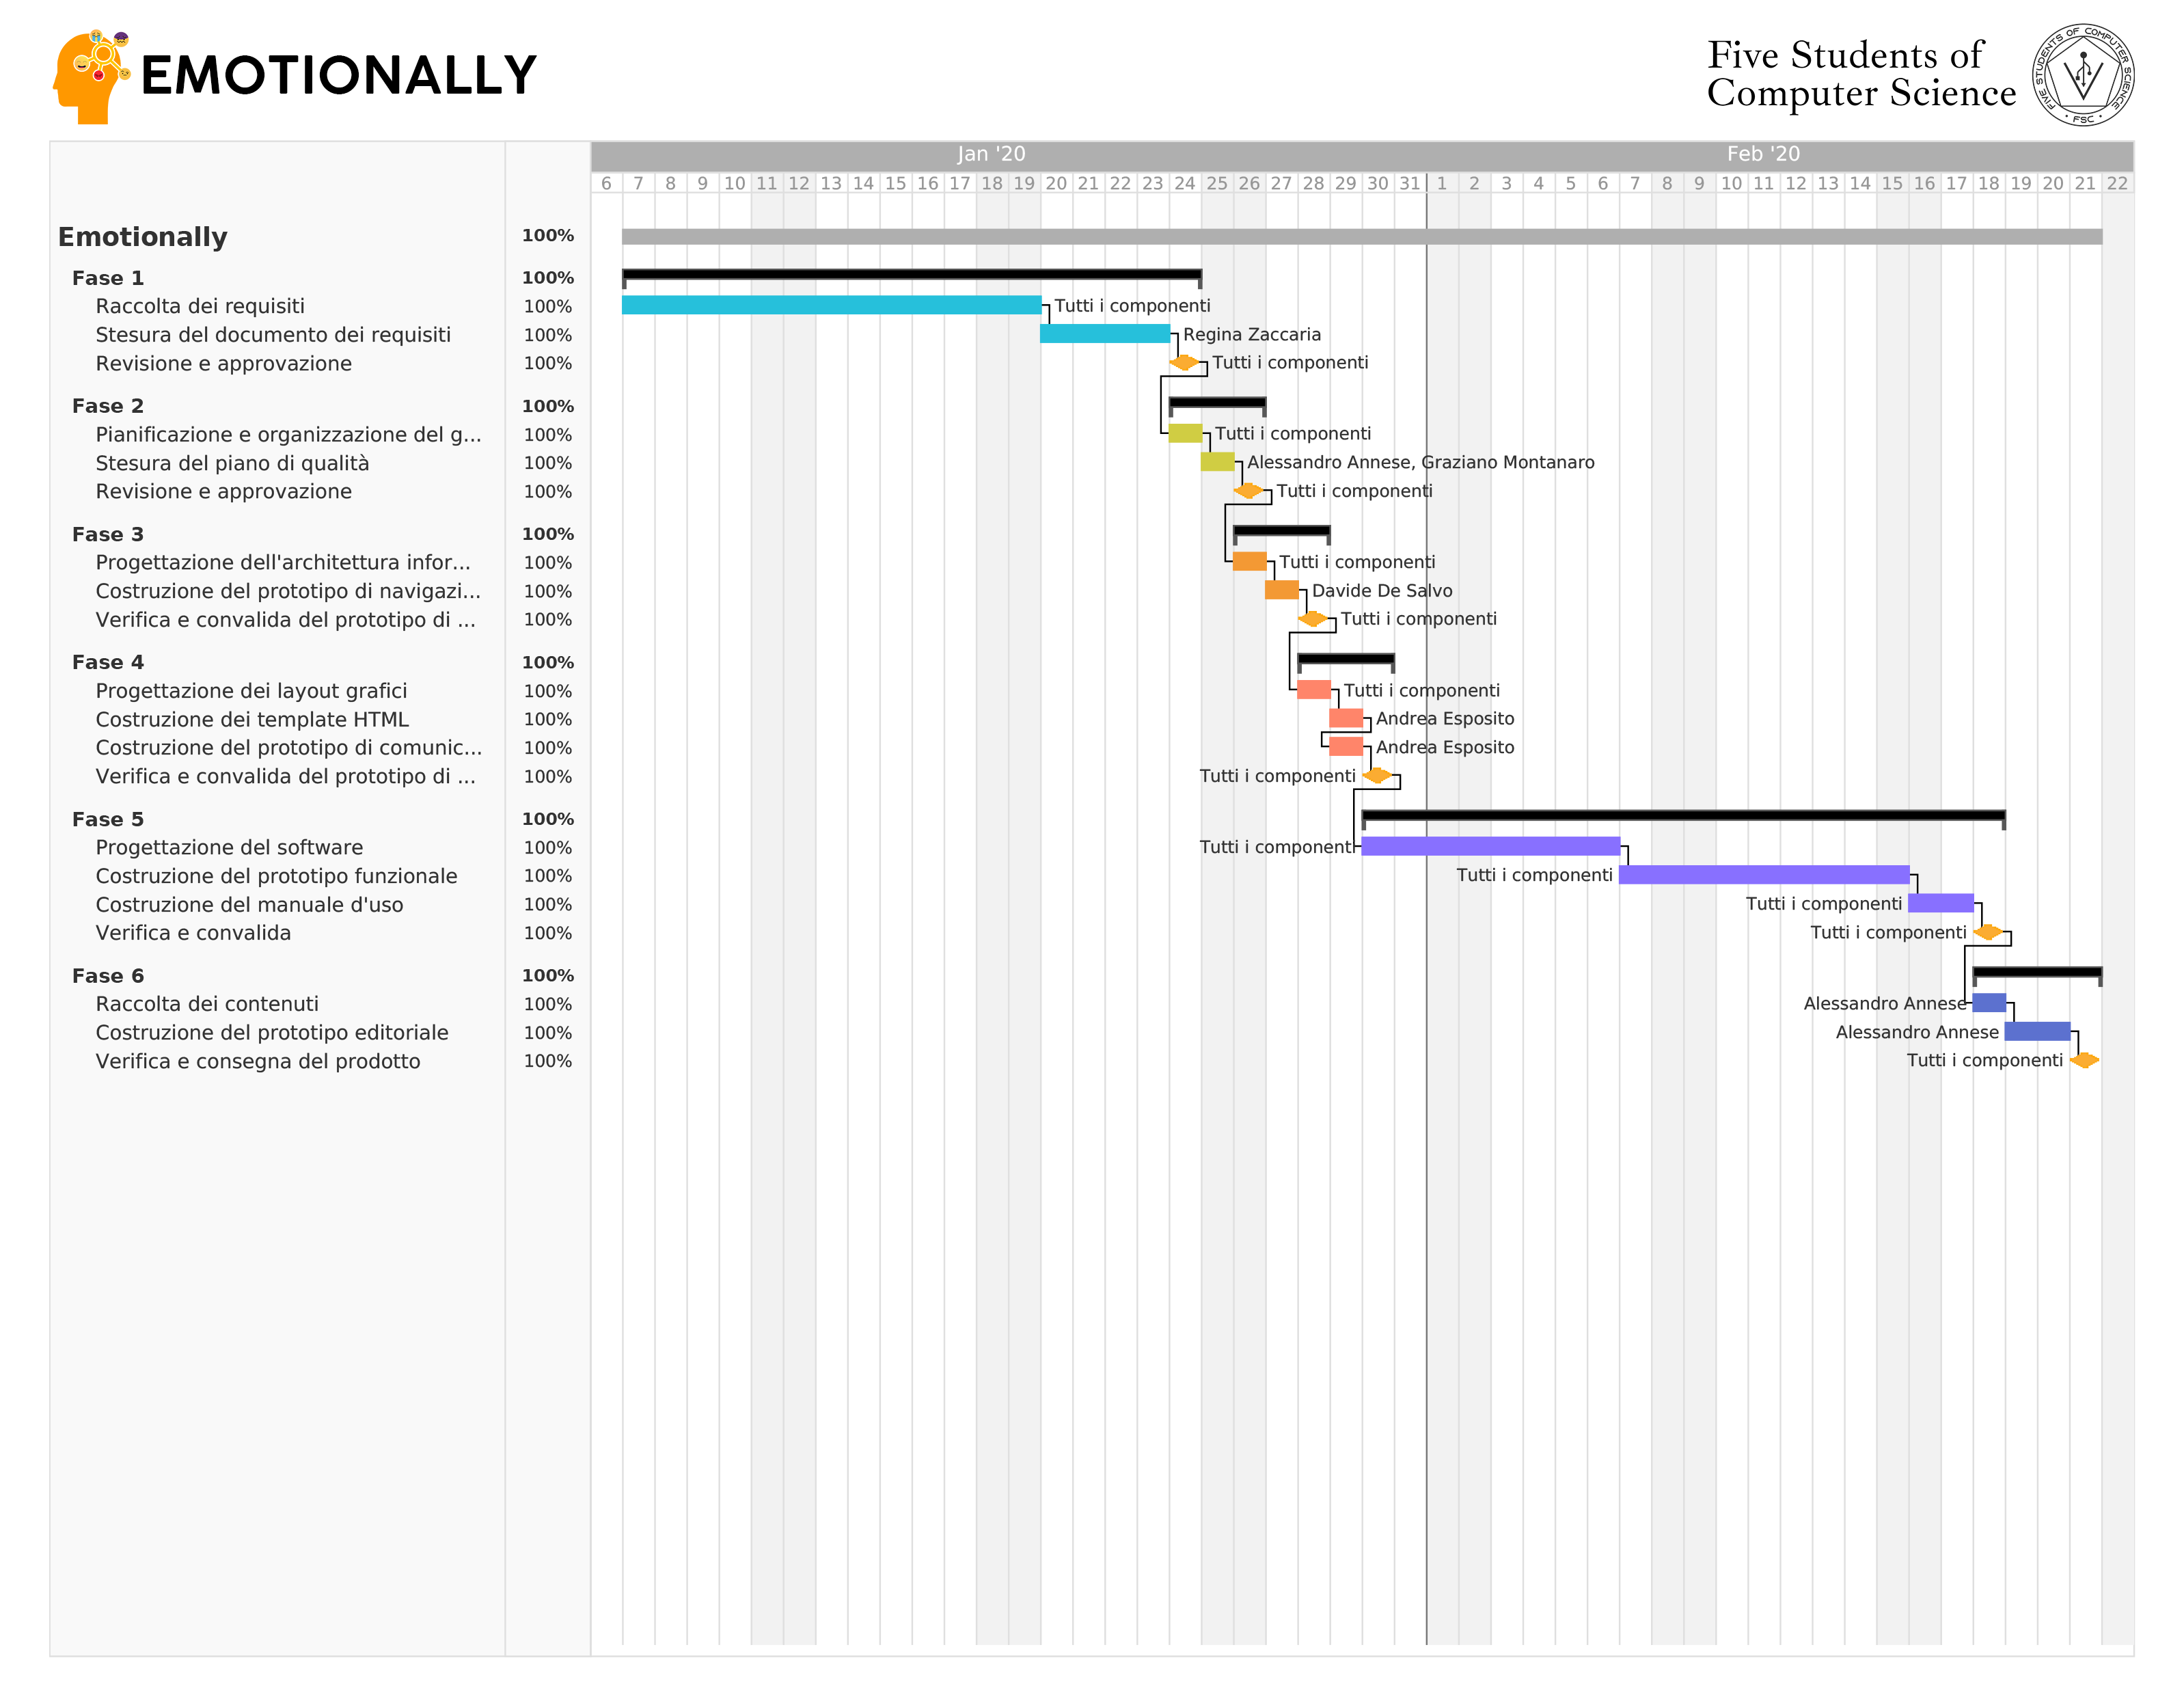
\includegraphics[height=11.5cm, frame]{images/gantt.png}

\section{Organizzazione del gruppo}\label{sec:organizzazione-gruppo}
Il gruppo, dopo essersi riunito in un brainsorming iniziale, ha deciso di 
dividersi in maniera modulare assegnando ad ogni componente un compito 
specifico.\\
In ogni fase, tutti i componenti del gruppo si riuniscono per una 
pianificazione iniziale e, alla fine di essa, si occupano  di verificare e 
convalidare il lavoro svolto.\\
Di seguito viene riportata la suddivisione dei compiti:

\begin{itemize}
	\item \textbf{Fase 1}\\
	In questa fase è prevista, oltre alla raccolta dei requisiti effettuata da 
	tutto il team, la stesura del documento dei requisiti. Quest'ultima è stata 
	assegnata a \textit{Regina Zaccaria}. Alla stesura hanno partecipato 
	\textit{Davide De Salvo} che ha realizzato le gabbie di massima del sito, 
	\textit{Alessandro Annese} che si è occupato della progettazione 
	concettuale del database e \textit{Andrea Esposito} che ha sistemato alcuni 
	errori grafici dei diagrammi, tabelle e gabbie logiche. 
	
	Il termine della fase è stato fissato per il 24/01/2020.
	\item \textbf{Fase 2}\\
	La stesura del piano di qualità è stata assegnata a \textit{Alessandro 
	Annese} e \textit{Graziano Montanaro}.
	
	Il termine della fase è stato fissato per il 26/01/2020.
	\item \textbf{Fase 3}\\
	La creazione del prototipo di navigazione è stata effettuata da 
	\textit{Davide De Salvo}. Il prototipo è stato realizzato con \texttt{Adobe 
	XD}.
	
	Il termine della fase è stato fissato per il 28/01/2020.
	\item \textbf{Fase 4}\\
	La costruzione dei template di base in \texttt{HTML} e del prototipo di 
	comunicazione è stata affidata a \textit{Andrea Esposito}.
	
	Il termine della fase è stato fissato per il 30/01/2020.
	\item \textbf{Fase 5}\\
	In questa fase si è progettato il software costruendo il prototipo 
	funzionale e, successivamente, si è redatto il manuale d'uso. Tutti i 
	membri del team si sono occupati di completare l'intera fase.
	
	Il termine della fase è stato fissato per il 18/02/2020.
	\item \textbf{Fase 6}\\
	La raccolta dei contenuti e successiva creazione del prototipo editoriale 
	sono stati affidati a \textit{Alessandro Annese}. Successivamente al 
	completamento della fase si è occupato anche di effettuare la consegna del 
	prototipo con la relativa documentazione al committente.
	
	Il termine della fase e relativa consegna del prodotto è fissato per il 
	21/02/2020.
\end{itemize}



% Copyright (c)  2019  FSC.
% Permission is granted to copy, distribute and/or modify this document
% under the terms of the GNU Free Documentation License, Version 1.3
% or any later version published by the Free Software Foundation;
% with no Invariant Sections, no Front-Cover Texts, and no Back-Cover Texts.
% A copy of the license is included in the section entitled "GNU
% Free Documentation License".

\part{Documento di progettazione}\label{part:documento-progettazione}

% Copyright (c)  2019  FSC.
% Permission is granted to copy, distribute and/or modify this document
% under the terms of the GNU Free Documentation License, Version 1.3
% or any later version published by the Free Software Foundation;
% with no Invariant Sections, no Front-Cover Texts, and no Back-Cover Texts.
% A copy of the license is included in the section entitled "GNU
% Free Documentation License".

\chapter{Web Design}\label{chap:web-design}
In questo capitolo viene illustrata la fase di web design.

Nel dettaglio, vengono mostrati i diagrammi relativi alla mappa del sito, gli 
storyboad delle pagine e i relativi prototipi di navigazione.

\section{Mappa del sito}\label{sec:mappa-sito}
La seguente mappa è la rappresentazione dei percorsi di navigazione del sito in 
un contesto generale.

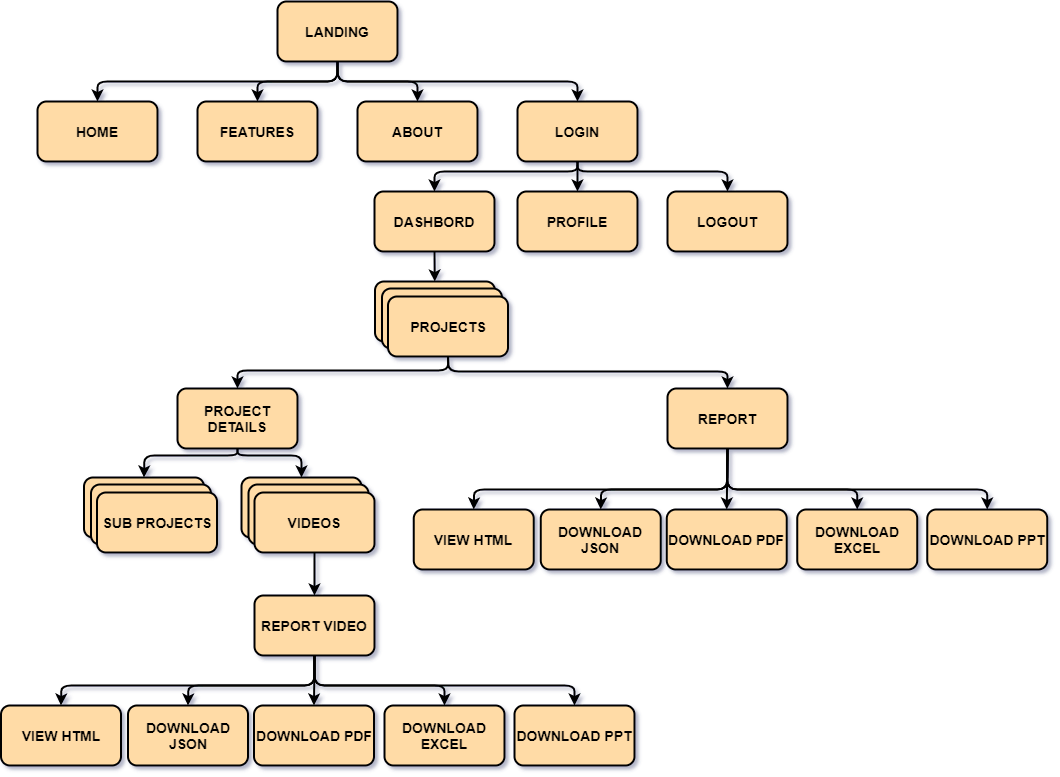
\includegraphics{images/mappa-sito.png}

\section{Storyboard}\label{sec:storyboard}
Gli storyboard sono la rappresentazione di particolari sequenze di navigazione 
del sito, accompagnata da una sintetica descrizione.

\input{images/storyboard.tex}

\section{Prototipo di navigazione}\label{sec:prototipo-navigazione}
È un prototipo piuttosto rudimentale completamente navigabile. Le pagine sono 
costituite dalla sola gabbia logica, in bianco e nero, senza grafica, senza 
contenuti informativi e il <<testo fittizio>> inserito nella gabbia logica.

\input{images/gabbia-logica.tex}


% Copyright (c)  2019  FSC.
% Permission is granted to copy, distribute and/or modify this document
% under the terms of the GNU Free Documentation License, Version 1.3
% or any later version published by the Free Software Foundation;
% with no Invariant Sections, no Front-Cover Texts, and no Back-Cover Texts.
% A copy of the license is included in the section entitled "GNU
% Free Documentation License".

\chapter{Visual Design}\label{chap:visual-design}


\section{Layout grafici}\label{sec:layout-grafici}



% Copyright (c)  2019  FSC.
% Permission is granted to copy, distribute and/or modify this document
% under the terms of the GNU Free Documentation License, Version 1.3
% or any later version published by the Free Software Foundation;
% with no Invariant Sections, no Front-Cover Texts, and no Back-Cover Texts.
% A copy of the license is included in the section entitled "GNU
% Free Documentation License".

\chapter{Sviluppo del sito}\label{chap:sviluppo-sito}
In questa fase, vengono descritte in dettaglio le funzioni precisando gli 
scenari di esecuzione di tutti i casi d'uso introdotti nalla fase dei 
requisiti. Si sono costruiti dei diagrammi di navigazione attraverso i 
diagrammi per macchine a stati. 

\input{images/diagrammi-macchine-stati.tex}

\section{Struttura dei form}\label{sec:struttura-form}

\input{images/struttura-form.tex}

\section{Modello logico base di dati}\label{sec:modello-logico}

\begin{figure}[H]
	\centering
	\caption{Modello logico della base di dati del sistema.}
	\label{fig:logical-diagram}
	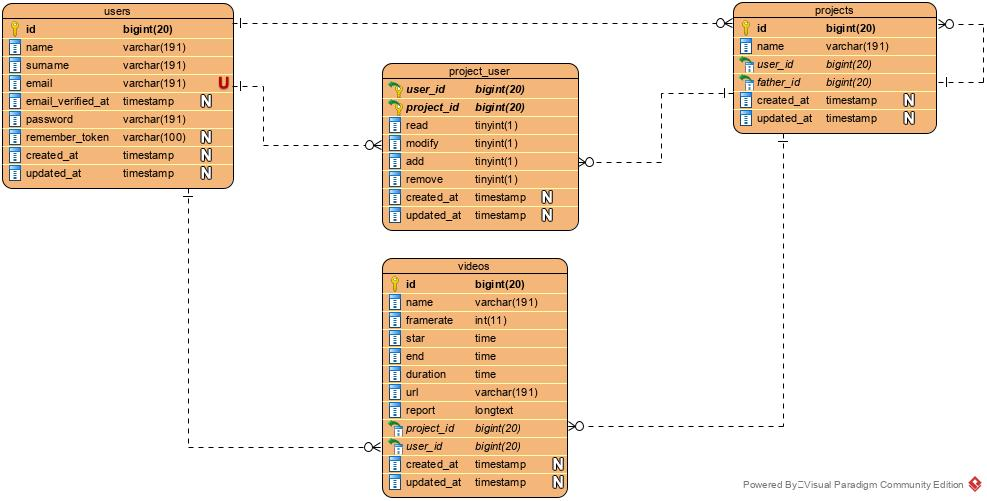
\includegraphics[width=\textwidth]{images/logical-diagram}
\end{figure}



% Copyright (c)  2019  FSC.
% Permission is granted to copy, distribute and/or modify this document
% under the terms of the GNU Free Documentation License, Version 1.3
% or any later version published by the Free Software Foundation;
% with no Invariant Sections, no Front-Cover Texts, and no Back-Cover Texts.
% A copy of the license is included in the section entitled "GNU
% Free Documentation License".

\chapter{Test}\label{chap:test}
Nella seguente sezione ci si concentra maggiormente sula fase di test del 
prodotto, analizzandone alcuni scenari di prova e integrandone le modifiche 
apportare in fase di alpha test e beta test.

\section{Scenari e casi di prova}\label{sec:scenari-casi-prova}
\paragraph{Scenari di prova per il caso d'uso 'Create project'}
Scenari di successo:
\begin{itemize}
	\item Inserimento progetto
\end{itemize}
Scenari di insuccesso:
\begin{itemize}
	\item Inserimento fallito a causa del nome scelto per il progetto già 
	esistente
\end{itemize}

\paragraph{Scenari di prova per il caso d'uso 'Update user data'}
Scenari di successo: 
\begin{itemize}
	\item Modificato il profilo
	\begin{itemize}
		\item Modificato il nome
		\item Modificato il cognome
		\item Modificata la password
	\end{itemize}
\end{itemize}
Scenari di insuccesso:
\begin{itemize}
	\item Modifica fallita a causa della vecchia password errata
	\item Modifica fallita a causa della non uguaglianza tra la nuova password 
	e conferma password (solo in caso si voglia modificare la password)
\end{itemize}

\section{Alpha test}\label{sec:alpha-test}
Non è stato condotto un vero e proprio alpha test, ma seguendo il modello 
basato sui prototipi successivi si sono effettuati i test in ogni fase della 
realizzazione di ogni singolo prototipo.

Per quanto riguarda la realizzazione del sistema, ad ogni item realizzato si 
sono effettuati i test di prova per convalidare la funzionalità testata 
evitando di portarsi uno o più errori fase della realizzazione.

\section{Beta test}
I seguenti dati riportati nella seguente tabella sono i problemi riscontrati 
dai soggetti intervistati (con dati anonimi) durante la fase di Beta Test, 
cercando di sollecitare il sistema nel maggior numero di modi possibili e 
verificando che esso si comporti secondo le aspettative.

\begin{table}[H]
	\resizebox{\textwidth}{!}{%
		\begin{tabular}{ccccccc}
			\textbf{Problema \#} & \textbf{Rilevato da} & \textbf{in data} & 
			\textbf{Caso d'uso} & \textbf{Descrizione del 
				problema}                                                       
				        
				                                         &
			\textbf{Gravità} & \textbf{Risolto in data} \\
			1                   & Soggetto 1           & 20/02/202        & 
			Upload 
			video        & \begin{tabular}[c]{@{}c@{}}Il sistema, se avviato 
			con 
				Google \\ Chrome, non permette l'inserimento \\ di video in 
				real 
				time\end{tabular} & 3                & -                        
				\\
			1                   & Soggetto 2           & 21/02/2020       & 
			Upload 
			video        & \begin{tabular}[c]{@{}c@{}}Il sistema, se avviato 
			con 
				Google \\ Chrome, non permette l'inserimento \\ di video in 
				real 
				time\end{tabular} & 3                & -                        
				\\
			2                   & Soggetto 4           & 21/02/2020       & 
			View 
			report         & \begin{tabular}[c]{@{}c@{}}Ogni tanto, anche se 
			non ci 
				sono \\ video, nel report si creano grafici\\ valorizzati a 
				0\end{tabular}        & 1                & 
				-                       
		\end{tabular}	
	}
\end{table}

Gravità:
	\begin{enumerate}
		\item problema molto lieve; può essere risolto dopo la pubblicazione 
		del sito
		\item problema lieve, da risolvere prima della pubblicazione del sito
		\item problema grave ma bypassabile; non pregiudica l'uso del sito
		\item problema bloccante, impedisce l'uso della funzione
	\end{enumerate}

\paragraph{Note} Il problema \textbf{\#1} è dovuto a un bug 
(\url{https://bugs.chromium.org/p/chromium/issues/detail?id=642012}) presente 
nel 
browser Chromium, su cui Google Chrome è basato, che non memorizza i metadati 
dei video WebM, rendendoli quindi non riproducibili. Come 
già riportato nei requisiti di usabilità, per il funzionamento corretto del 
sistema, è consigliabile l'utilizzo di Firefox.


\backmatter
\printbibliography[heading=bibintoc]
\appendix
\part*{Appendice}\label{part:appendice}
\addcontentsline{toc}{part}{Appendice}
\chapter*{GNU Free Documentation License}
\phantomsection  % so hyperref creates bookmarks
\addcontentsline{toc}{chapter}{GNU Free Documentation License}
% \label{label_fdl}

 \begin{center}

       Version 1.3, 3 November 2008


 Copyright \copyright{} 2000, 2001, 2002, 2007, 2008  Free Software Foundation, Inc.

 \bigskip

     \texttt{<https://fsf.org/>}

 \bigskip

 Everyone is permitted to copy and distribute verbatim copies
 of this license document, but changing it is not allowed.
\end{center}


\begin{center}
{\bf\large Preamble}
\end{center}

The purpose of this License is to make a manual, textbook, or other
functional and useful document ``free'' in the sense of freedom: to
assure everyone the effective freedom to copy and redistribute it,
with or without modifying it, either commercially or noncommercially.
Secondarily, this License preserves for the author and publisher a way
to get credit for their work, while not being considered responsible
for modifications made by others.

This License is a kind of ``copyleft'', which means that derivative
works of the document must themselves be free in the same sense.  It
complements the GNU General Public License, which is a copyleft
license designed for free software.

We have designed this License in order to use it for manuals for free
software, because free software needs free documentation: a free
program should come with manuals providing the same freedoms that the
software does.  But this License is not limited to software manuals;
it can be used for any textual work, regardless of subject matter or
whether it is published as a printed book.  We recommend this License
principally for works whose purpose is instruction or reference.


\begin{center}
{\Large\bf 1. APPLICABILITY AND DEFINITIONS\par}
\phantomsection
\addcontentsline{toc}{section}{1. APPLICABILITY AND DEFINITIONS}
\end{center}

This License applies to any manual or other work, in any medium, that
contains a notice placed by the copyright holder saying it can be
distributed under the terms of this License.  Such a notice grants a
world-wide, royalty-free license, unlimited in duration, to use that
work under the conditions stated herein.  The ``\textbf{Document}'', below,
refers to any such manual or work.  Any member of the public is a
licensee, and is addressed as ``\textbf{you}''.  You accept the license if you
copy, modify or distribute the work in a way requiring permission
under copyright law.

A ``\textbf{Modified Version}'' of the Document means any work containing the
Document or a portion of it, either copied verbatim, or with
modifications and/or translated into another language.

A ``\textbf{Secondary Section}'' is a named appendix or a front-matter section of
the Document that deals exclusively with the relationship of the
publishers or authors of the Document to the Document's overall subject
(or to related matters) and contains nothing that could fall directly
within that overall subject.  (Thus, if the Document is in part a
textbook of mathematics, a Secondary Section may not explain any
mathematics.)  The relationship could be a matter of historical
connection with the subject or with related matters, or of legal,
commercial, philosophical, ethical or political position regarding
them.

The ``\textbf{Invariant Sections}'' are certain Secondary Sections whose titles
are designated, as being those of Invariant Sections, in the notice
that says that the Document is released under this License.  If a
section does not fit the above definition of Secondary then it is not
allowed to be designated as Invariant.  The Document may contain zero
Invariant Sections.  If the Document does not identify any Invariant
Sections then there are none.

The ``\textbf{Cover Texts}'' are certain short passages of text that are listed,
as Front-Cover Texts or Back-Cover Texts, in the notice that says that
the Document is released under this License.  A Front-Cover Text may
be at most 5 words, and a Back-Cover Text may be at most 25 words.

A ``\textbf{Transparent}'' copy of the Document means a machine-readable copy,
represented in a format whose specification is available to the
general public, that is suitable for revising the document
straightforwardly with generic text editors or (for images composed of
pixels) generic paint programs or (for drawings) some widely available
drawing editor, and that is suitable for input to text formatters or
for automatic translation to a variety of formats suitable for input
to text formatters.  A copy made in an otherwise Transparent file
format whose markup, or absence of markup, has been arranged to thwart
or discourage subsequent modification by readers is not Transparent.
An image format is not Transparent if used for any substantial amount
of text.  A copy that is not ``Transparent'' is called ``\textbf{Opaque}''.

Examples of suitable formats for Transparent copies include plain
ASCII without markup, Texinfo input format, LaTeX input format, SGML
or XML using a publicly available DTD, and standard-conforming simple
HTML, PostScript or PDF designed for human modification.  Examples of
transparent image formats include PNG, XCF and JPG.  Opaque formats
include proprietary formats that can be read and edited only by
proprietary word processors, SGML or XML for which the DTD and/or
processing tools are not generally available, and the
machine-generated HTML, PostScript or PDF produced by some word
processors for output purposes only.

The ``\textbf{Title Page}'' means, for a printed book, the title page itself,
plus such following pages as are needed to hold, legibly, the material
this License requires to appear in the title page.  For works in
formats which do not have any title page as such, ``Title Page'' means
the text near the most prominent appearance of the work's title,
preceding the beginning of the body of the text.

The ``\textbf{publisher}'' means any person or entity that distributes
copies of the Document to the public.

A section ``\textbf{Entitled XYZ}'' means a named subunit of the Document whose
title either is precisely XYZ or contains XYZ in parentheses following
text that translates XYZ in another language.  (Here XYZ stands for a
specific section name mentioned below, such as ``\textbf{Acknowledgements}'',
``\textbf{Dedications}'', ``\textbf{Endorsements}'', or ``\textbf{History}''.)
To ``\textbf{Preserve the Title}''
of such a section when you modify the Document means that it remains a
section ``Entitled XYZ'' according to this definition.

The Document may include Warranty Disclaimers next to the notice which
states that this License applies to the Document.  These Warranty
Disclaimers are considered to be included by reference in this
License, but only as regards disclaiming warranties: any other
implication that these Warranty Disclaimers may have is void and has
no effect on the meaning of this License.


\begin{center}
{\Large\bf 2. VERBATIM COPYING\par}
\phantomsection
\addcontentsline{toc}{section}{2. VERBATIM COPYING}
\end{center}

You may copy and distribute the Document in any medium, either
commercially or noncommercially, provided that this License, the
copyright notices, and the license notice saying this License applies
to the Document are reproduced in all copies, and that you add no other
conditions whatsoever to those of this License.  You may not use
technical measures to obstruct or control the reading or further
copying of the copies you make or distribute.  However, you may accept
compensation in exchange for copies.  If you distribute a large enough
number of copies you must also follow the conditions in section~3.

You may also lend copies, under the same conditions stated above, and
you may publicly display copies.


\begin{center}
{\Large\bf 3. COPYING IN QUANTITY\par}
\phantomsection
\addcontentsline{toc}{section}{3. COPYING IN QUANTITY}
\end{center}


If you publish printed copies (or copies in media that commonly have
printed covers) of the Document, numbering more than 100, and the
Document's license notice requires Cover Texts, you must enclose the
copies in covers that carry, clearly and legibly, all these Cover
Texts: Front-Cover Texts on the front cover, and Back-Cover Texts on
the back cover.  Both covers must also clearly and legibly identify
you as the publisher of these copies.  The front cover must present
the full title with all words of the title equally prominent and
visible.  You may add other material on the covers in addition.
Copying with changes limited to the covers, as long as they preserve
the title of the Document and satisfy these conditions, can be treated
as verbatim copying in other respects.

If the required texts for either cover are too voluminous to fit
legibly, you should put the first ones listed (as many as fit
reasonably) on the actual cover, and continue the rest onto adjacent
pages.

If you publish or distribute Opaque copies of the Document numbering
more than 100, you must either include a machine-readable Transparent
copy along with each Opaque copy, or state in or with each Opaque copy
a computer-network location from which the general network-using
public has access to download using public-standard network protocols
a complete Transparent copy of the Document, free of added material.
If you use the latter option, you must take reasonably prudent steps,
when you begin distribution of Opaque copies in quantity, to ensure
that this Transparent copy will remain thus accessible at the stated
location until at least one year after the last time you distribute an
Opaque copy (directly or through your agents or retailers) of that
edition to the public.

It is requested, but not required, that you contact the authors of the
Document well before redistributing any large number of copies, to give
them a chance to provide you with an updated version of the Document.


\begin{center}
{\Large\bf 4. MODIFICATIONS\par}
\phantomsection
\addcontentsline{toc}{section}{4. MODIFICATIONS}
\end{center}

You may copy and distribute a Modified Version of the Document under
the conditions of sections 2 and 3 above, provided that you release
the Modified Version under precisely this License, with the Modified
Version filling the role of the Document, thus licensing distribution
and modification of the Modified Version to whoever possesses a copy
of it.  In addition, you must do these things in the Modified Version:

\begin{itemize}
\item[A.]
   Use in the Title Page (and on the covers, if any) a title distinct
   from that of the Document, and from those of previous versions
   (which should, if there were any, be listed in the History section
   of the Document).  You may use the same title as a previous version
   if the original publisher of that version gives permission.

\item[B.]
   List on the Title Page, as authors, one or more persons or entities
   responsible for authorship of the modifications in the Modified
   Version, together with at least five of the principal authors of the
   Document (all of its principal authors, if it has fewer than five),
   unless they release you from this requirement.

\item[C.]
   State on the Title page the name of the publisher of the
   Modified Version, as the publisher.

\item[D.]
   Preserve all the copyright notices of the Document.

\item[E.]
   Add an appropriate copyright notice for your modifications
   adjacent to the other copyright notices.

\item[F.]
   Include, immediately after the copyright notices, a license notice
   giving the public permission to use the Modified Version under the
   terms of this License, in the form shown in the Addendum below.

\item[G.]
   Preserve in that license notice the full lists of Invariant Sections
   and required Cover Texts given in the Document's license notice.

\item[H.]
   Include an unaltered copy of this License.

\item[I.]
   Preserve the section Entitled ``History'', Preserve its Title, and add
   to it an item stating at least the title, year, new authors, and
   publisher of the Modified Version as given on the Title Page.  If
   there is no section Entitled ``History'' in the Document, create one
   stating the title, year, authors, and publisher of the Document as
   given on its Title Page, then add an item describing the Modified
   Version as stated in the previous sentence.

\item[J.]
   Preserve the network location, if any, given in the Document for
   public access to a Transparent copy of the Document, and likewise
   the network locations given in the Document for previous versions
   it was based on.  These may be placed in the ``History'' section.
   You may omit a network location for a work that was published at
   least four years before the Document itself, or if the original
   publisher of the version it refers to gives permission.

\item[K.]
   For any section Entitled ``Acknowledgements'' or ``Dedications'',
   Preserve the Title of the section, and preserve in the section all
   the substance and tone of each of the contributor acknowledgements
   and/or dedications given therein.

\item[L.]
   Preserve all the Invariant Sections of the Document,
   unaltered in their text and in their titles.  Section numbers
   or the equivalent are not considered part of the section titles.

\item[M.]
   Delete any section Entitled ``Endorsements''.  Such a section
   may not be included in the Modified Version.

\item[N.]
   Do not retitle any existing section to be Entitled ``Endorsements''
   or to conflict in title with any Invariant Section.

\item[O.]
   Preserve any Warranty Disclaimers.
\end{itemize}

If the Modified Version includes new front-matter sections or
appendices that qualify as Secondary Sections and contain no material
copied from the Document, you may at your option designate some or all
of these sections as invariant.  To do this, add their titles to the
list of Invariant Sections in the Modified Version's license notice.
These titles must be distinct from any other section titles.

You may add a section Entitled ``Endorsements'', provided it contains
nothing but endorsements of your Modified Version by various
parties---for example, statements of peer review or that the text has
been approved by an organization as the authoritative definition of a
standard.

You may add a passage of up to five words as a Front-Cover Text, and a
passage of up to 25 words as a Back-Cover Text, to the end of the list
of Cover Texts in the Modified Version.  Only one passage of
Front-Cover Text and one of Back-Cover Text may be added by (or
through arrangements made by) any one entity.  If the Document already
includes a cover text for the same cover, previously added by you or
by arrangement made by the same entity you are acting on behalf of,
you may not add another; but you may replace the old one, on explicit
permission from the previous publisher that added the old one.

The author(s) and publisher(s) of the Document do not by this License
give permission to use their names for publicity for or to assert or
imply endorsement of any Modified Version.


\begin{center}
{\Large\bf 5. COMBINING DOCUMENTS\par}
\phantomsection
\addcontentsline{toc}{section}{5. COMBINING DOCUMENTS}
\end{center}


You may combine the Document with other documents released under this
License, under the terms defined in section~4 above for modified
versions, provided that you include in the combination all of the
Invariant Sections of all of the original documents, unmodified, and
list them all as Invariant Sections of your combined work in its
license notice, and that you preserve all their Warranty Disclaimers.

The combined work need only contain one copy of this License, and
multiple identical Invariant Sections may be replaced with a single
copy.  If there are multiple Invariant Sections with the same name but
different contents, make the title of each such section unique by
adding at the end of it, in parentheses, the name of the original
author or publisher of that section if known, or else a unique number.
Make the same adjustment to the section titles in the list of
Invariant Sections in the license notice of the combined work.

In the combination, you must combine any sections Entitled ``History''
in the various original documents, forming one section Entitled
``History''; likewise combine any sections Entitled ``Acknowledgements'',
and any sections Entitled ``Dedications''.  You must delete all sections
Entitled ``Endorsements''.

\begin{center}
{\Large\bf 6. COLLECTIONS OF DOCUMENTS\par}
\phantomsection
\addcontentsline{toc}{section}{6. COLLECTIONS OF DOCUMENTS}
\end{center}

You may make a collection consisting of the Document and other documents
released under this License, and replace the individual copies of this
License in the various documents with a single copy that is included in
the collection, provided that you follow the rules of this License for
verbatim copying of each of the documents in all other respects.

You may extract a single document from such a collection, and distribute
it individually under this License, provided you insert a copy of this
License into the extracted document, and follow this License in all
other respects regarding verbatim copying of that document.


\begin{center}
{\Large\bf 7. AGGREGATION WITH INDEPENDENT WORKS\par}
\phantomsection
\addcontentsline{toc}{section}{7. AGGREGATION WITH INDEPENDENT WORKS}
\end{center}


A compilation of the Document or its derivatives with other separate
and independent documents or works, in or on a volume of a storage or
distribution medium, is called an ``aggregate'' if the copyright
resulting from the compilation is not used to limit the legal rights
of the compilation's users beyond what the individual works permit.
When the Document is included in an aggregate, this License does not
apply to the other works in the aggregate which are not themselves
derivative works of the Document.

If the Cover Text requirement of section~3 is applicable to these
copies of the Document, then if the Document is less than one half of
the entire aggregate, the Document's Cover Texts may be placed on
covers that bracket the Document within the aggregate, or the
electronic equivalent of covers if the Document is in electronic form.
Otherwise they must appear on printed covers that bracket the whole
aggregate.


\begin{center}
{\Large\bf 8. TRANSLATION\par}
\phantomsection
\addcontentsline{toc}{section}{8. TRANSLATION}
\end{center}


Translation is considered a kind of modification, so you may
distribute translations of the Document under the terms of section~4.
Replacing Invariant Sections with translations requires special
permission from their copyright holders, but you may include
translations of some or all Invariant Sections in addition to the
original versions of these Invariant Sections.  You may include a
translation of this License, and all the license notices in the
Document, and any Warranty Disclaimers, provided that you also include
the original English version of this License and the original versions
of those notices and disclaimers.  In case of a disagreement between
the translation and the original version of this License or a notice
or disclaimer, the original version will prevail.

If a section in the Document is Entitled ``Acknowledgements'',
``Dedications'', or ``History'', the requirement (section~4) to Preserve
its Title (section~1) will typically require changing the actual
title.


\begin{center}
{\Large\bf 9. TERMINATION\par}
\phantomsection
\addcontentsline{toc}{section}{9. TERMINATION}
\end{center}


You may not copy, modify, sublicense, or distribute the Document
except as expressly provided under this License.  Any attempt
otherwise to copy, modify, sublicense, or distribute it is void, and
will automatically terminate your rights under this License.

However, if you cease all violation of this License, then your license
from a particular copyright holder is reinstated (a) provisionally,
unless and until the copyright holder explicitly and finally
terminates your license, and (b) permanently, if the copyright holder
fails to notify you of the violation by some reasonable means prior to
60 days after the cessation.

Moreover, your license from a particular copyright holder is
reinstated permanently if the copyright holder notifies you of the
violation by some reasonable means, this is the first time you have
received notice of violation of this License (for any work) from that
copyright holder, and you cure the violation prior to 30 days after
your receipt of the notice.

Termination of your rights under this section does not terminate the
licenses of parties who have received copies or rights from you under
this License.  If your rights have been terminated and not permanently
reinstated, receipt of a copy of some or all of the same material does
not give you any rights to use it.


\begin{center}
{\Large\bf 10. FUTURE REVISIONS OF THIS LICENSE\par}
\phantomsection
\addcontentsline{toc}{section}{10. FUTURE REVISIONS OF THIS LICENSE}
\end{center}


The Free Software Foundation may publish new, revised versions
of the GNU Free Documentation License from time to time.  Such new
versions will be similar in spirit to the present version, but may
differ in detail to address new problems or concerns.  See
\texttt{https://www.gnu.org/licenses/}.

Each version of the License is given a distinguishing version number.
If the Document specifies that a particular numbered version of this
License ``or any later version'' applies to it, you have the option of
following the terms and conditions either of that specified version or
of any later version that has been published (not as a draft) by the
Free Software Foundation.  If the Document does not specify a version
number of this License, you may choose any version ever published (not
as a draft) by the Free Software Foundation.  If the Document
specifies that a proxy can decide which future versions of this
License can be used, that proxy's public statement of acceptance of a
version permanently authorizes you to choose that version for the
Document.


\begin{center}
{\Large\bf 11. RELICENSING\par}
\phantomsection
\addcontentsline{toc}{section}{11. RELICENSING}
\end{center}


``Massive Multiauthor Collaboration Site'' (or ``MMC Site'') means any
World Wide Web server that publishes copyrightable works and also
provides prominent facilities for anybody to edit those works.  A
public wiki that anybody can edit is an example of such a server.  A
``Massive Multiauthor Collaboration'' (or ``MMC'') contained in the
site means any set of copyrightable works thus published on the MMC
site.

``CC-BY-SA'' means the Creative Commons Attribution-Share Alike 3.0
license published by Creative Commons Corporation, a not-for-profit
corporation with a principal place of business in San Francisco,
California, as well as future copyleft versions of that license
published by that same organization.

``Incorporate'' means to publish or republish a Document, in whole or
in part, as part of another Document.

An MMC is ``eligible for relicensing'' if it is licensed under this
License, and if all works that were first published under this License
somewhere other than this MMC, and subsequently incorporated in whole
or in part into the MMC, (1) had no cover texts or invariant sections,
and (2) were thus incorporated prior to November 1, 2008.

The operator of an MMC Site may republish an MMC contained in the site
under CC-BY-SA on the same site at any time before August 1, 2009,
provided the MMC is eligible for relicensing.


\begin{center}
{\Large\bf ADDENDUM: How to use this License for your documents\par}
\phantomsection
\addcontentsline{toc}{section}{ADDENDUM: How to use this License for your documents}
\end{center}

To use this License in a document you have written, include a copy of
the License in the document and put the following copyright and
license notices just after the title page:

\bigskip
\begin{quote}
    Copyright \copyright{}  YEAR  YOUR NAME.
    Permission is granted to copy, distribute and/or modify this document
    under the terms of the GNU Free Documentation License, Version 1.3
    or any later version published by the Free Software Foundation;
    with no Invariant Sections, no Front-Cover Texts, and no Back-Cover Texts.
    A copy of the license is included in the section entitled ``GNU
    Free Documentation License''.
\end{quote}
\bigskip

If you have Invariant Sections, Front-Cover Texts and Back-Cover Texts,
replace the ``with \dots\ Texts.''\ line with this:

\bigskip
\begin{quote}
    with the Invariant Sections being LIST THEIR TITLES, with the
    Front-Cover Texts being LIST, and with the Back-Cover Texts being LIST.
\end{quote}
\bigskip

If you have Invariant Sections without Cover Texts, or some other
combination of the three, merge those two alternatives to suit the
situation.

If your document contains nontrivial examples of program code, we
recommend releasing these examples in parallel under your choice of
free software license, such as the GNU General Public License,
to permit their use in free software.
\end{document}